\chapter{Introduction}

\emph{"Statistics ist the explanation of variance in the light of what remains
unexplained."}

\vspace{5 mm}

Statistics was originally invented - as so many other things - by the famous mathematician C.F. Gauss, who said about his own work \emph{"Ich habe fleissig sein m\"ussen; wer es gleichfalls ist, wird eben so weit kommen"}. Even if your aspirations are not that high, you can get a lot out of statistics. In fact, if your work with real data, you probably won't be able to avoid it. Statistics can

\begin{itemize}
  \item Describe variation.
  \item Make quantitative statements about populations.
  \item Make predictions.
\end{itemize}

\textbf{Books: }There are a number of good books about statistics. My favorite is \cite{altman99}: it does not talk a lot about computers and modeling, but gives you a terrific introduction into the field. Many formulations and examples in this manuscript have been taken from that book. A more modern book, which is more voluminous and in my opionion a bit harder to read, is \cite{Riffenburgh2012}. If you are interested in a simple introduction to modern regression modeling, check out \cite{Kaplan2009}. A very good introduction to “Generalized Linear Models” is \cite{Dobson2008}. If you know your basic statistics, this is a good, advanced starter into statistical modeling.

\vspace{5 mm}

\textbf{WWW: }On the web, you find good very extensive statistics information in English under
\begin{itemize}
    \item \url{http://www.statsref.com/}
    \item \url{http://www.vassarstats.net/}
    \item \url{http://udel.edu/~mcdonald/statintro.html}
    \item \url{http://onlinestatbook.com/2/index.html}
\end{itemize}

 A good German webpage on statistics and regulatory issues is \url{http://www.reiter1.com/}.

\vspace{5 mm}

\textbf{Exercises: }Many examples are already solved in the text. For the use in lectures (or for self-test), additional exercises are provided at the end of most chapters. For lecturers, solutions to these exercises can be provided on demand. Please contact me directly for that via email.

\section{Why Statistics?}

Statistics will help you to
\begin{itemize}
  \item Clarify the question.
  \item Identify the variable and the measure of that variable that will answer that question.
  \item Determine the required sample size.
  \item Find the correct analysis for your data.
  \item Make predictions based on your data.
\end{itemize}

Without statistics, your interpretation of your data can be massively flawed. Take for example the estimated number of German tanks during World War II, also known as the \emph{German tank problem} (\url{http://en.wikipedia.org/wiki/German_tank_problem}): from standard intelligence data, the estimate for the number of German tanks produced per month was $1550$; in contrast, the statistical estimate from the tanks observed led to a number of $327$, which was very close to the actual production number of $342$.

\section{What you should already know}

From previous courses on math, quality control, signal analysis, etc., you are probably already familiar with a number of statistical concepts. While they will be dealt with in detail later on, let me list them here to make sure we start at the same level:

\begin{itemize}
  \item mean
  \item median
  \item mode
  \item standard deviation
  \item variance
  \item confidence intervals
  \item t-test
  \item boxplot
  \item normal distribution
  \item regression coefficient
  \item coefficient of determination
\end{itemize}

\section{Projects}

The biggest problems in statistics do \emph{not} arise from a faulty analysis, but from a faulty experimental design. If you have a suitable topic of interest, you can select to do a project instead of the final exam. For this you will have to

\begin{enumerate}
  \item Read up on the problem.
  \item Design the study:

  \begin{enumerate}
    \item Determine the parameter to analyze.
    \item Decide on the requirements of the sample population.
    \item Plan the randomization.
    \item Decide which test you want to use for the analysis.
  \end{enumerate}

  \item Analyze some data.
  \item Generate the appropriate graphs.
  \item Write up a summary of your project.
\end{enumerate}

\section{Programming Matters}

\subsection{Python}


There are three reasons why I have decided to use Python for this lecture.

\begin{enumerate}
  \item It is the most elegant programming language that I know.
  \item It is free.
  \item It is powerful.
\end{enumerate}

I have not seen many books on Python that I really liked. My favorite introductory book is \cite{Harms2010}.
A good free book, which introduces Python with a focus on statistics, is \href{http://www.kevinsheppard.com/images/0/09/Python_introduction.pdf} {Introduction to Python for Econometrics, Statistics and Data Analysis, by Kevin Sheppard, Oxford University}.

In general, I suggest that you start out by installing a Python distribution which includes the most important libraries. Since I suggest that you use Python $>3.3$ for this course, \cite{pythonxy} (which comes complete with help) is currently not an option, since it is only available for Python 2.7. All the Python packages required for this course are now available for Python 3, so I don't see a good reason to stay with Python 2.7 . My favorites Python 3.3 distributions  are

\begin{enumerate}
    \item \cite{winpython} No admin-rights required.
    \item \cite{anaconda} From Continuum.
\end{enumerate}

which are very good starting points when you are using Windows. \emph{winpython} does not require administrator rights, and \emph{anaconda} is a more recent distribution, which is free for educational purposes.

Mac and Unix users should check out the installations tips from Johansson (see Table \ref{table:python}).

There are also many tutorials available on the internet (Table \ref{table:python}). Personally, most of the time I just google; thereby I stick primarily a) to the official pages, and b) to \url{http://stackoverflow.com/}. Also, I have found user groups surprisingly active and helpful!

\begin{table}

  \footnotesize{
  \centering
   \begin{tabular}{|l p{8 cm}|}
     \hline
     \url{http://scipy-lectures.github.com} & \emph{Python Scientific Lecture Notes.} Pretty comprehensive. \\     \url{http://www.scipy.org/NumPy\_for\_Matlab\_Users} & \emph{NumPy for Matlab Users} Start here if you have Matlab experience. \\
     \url {https://github.com/jrjohansson/scientific-python-lectures} & \emph{Lectures on scientific computing with Python.} Great ipython notebooks! \\     \url{http://docs.python.org/2/tutorial} & \emph{The Python tutorial.} The official introduction. \\
     \url{http://swaroopch.com/notes/python} & \emph{A Byte of Python.} Free book, very good at the introductory level. \\
     \url{http://learnpythonthehardway.org/book/} & \emph{Learn Python the Hard Way, 3rd Ed} A popular, free book that you can work through. \\
     \url{http://www.greenteapress.com/thinkpython} & \emph{ThinkPython.} Free book, for advanced programers. \\

     \hline
   \end{tabular}
   }
  \caption{Python on the WWW}\label{table:python}
\end{table}

If you decide to install things manually, you need the following modules in addition to the Python standard library:

\begin{itemize}
  \item \emph{ipython} ... For interactive work.
  \item \emph{numpy} ... For working with vectors and arrays.
  \item \emph{scipy} ... All the essential scientific algorithms, including those for statistics.
  \item \emph{matplotlib} ... The de-facto standard module for plotting and visualization.
  \item \emph{pandas} ... Adds \emph{DataFrames} (imagine powerful spreadsheets) to Python.
  \item \emph{patsy} ... For working with statistical formulas.
  \item \emph{statsmodels} ... For statistical modeling and advanced analysis.
  \item \emph{seaborn} ... For visualization of statistical data.
\end{itemize}

\subsubsection{Ipython}


Make sure that you have a good programming environment! Currently, my favorite way of programming is similar to my old Matlab style: I first get the individual steps worked out interactively in an \cite{ipython} \emph{qtconsole}. Ipython \index{general}{Python!ipython} provides interactive computing with Python, similar to the commandline in Matlab. It comes with a command history, interactive data visualization, command completion, and a lot of features that make it quick and easy to try out code.
When ipython is started in \emph{pylab mode} (which is the typical configuration), it automatically loads numpy and matplotlib.pyplot into the
active workspace, and provides a very convenient, Matlab-like programing environment. A very helpful new addition is the browser-based \emph{ipython
notebook}, with support for code, text, mathematical expressions, inline plots and other rich media. Please check out the links to the ipython
notebooks in this statistics introduction. I believe that it will  help you to get up to speed with python much more quickly.

And to write a program, I then go to either \emph{Spyder} (which is free) or \emph{Wing} (which is very good, but commercial). \emph{PyCharm} is another IDE with a good debugger, and has very good vim-emulation.

The flexibility of Python has the "disadvantage" that it can come in
different flavors or coding styles. When you know the different approaches,
they are great to use. But when you get started, it can be a bit confusing.
The following section from the Matplotlib documentation may help to clarify
these things:

\subsubsection{Matplotlib, pylab, and pyplot: how are they related?}

\textbf{Matplotlib}\index{general}{Python!Matplotlib} is the whole package; \emph{pylab} is a module in matplotlib that gets installed alongside matplotlib; and \emph{matplotlib.pyplot} is a module in matplotlib.

\textbf{Pyplot}\index{general}{Python!pyplot} provides the state-machine interface to the underlying plotting library in matplotlib. This means that figures and axes are implicitly and automatically created to achieve the desired plot. For example, calling plot from pyplot will automatically create the necessary figure and axes to achieve the desired plot. Setting a title will then automatically set that title to the current axes object:

\begin{lstlisting}
    import matplotlib.pyplot as plt

    plt.plot(arange(10))
    plt.title("Simple Plot")
    plt.show()
\end{lstlisting}

\textbf{Pylab}\index{general}{Python!pylab} combines the pyplot functionality (for plotting) with the numpy functionality (for mathematics and for working with arrays) in a single namespace, making that namespace (or environment) even more MATLAB-like. For example, one can call the sin and cos functions just like you could in MATLAB, as well as having all the features of pyplot.

The pyplot interface is generally preferred for non-interactive plotting (i.e., scripting). The pylab interface is convenient for interactive calculations and plotting, as it minimizes typing. Note that this is what you get if you use the ipython shell with the -pylab option, which imports everything from pylab and makes plotting fully interactive.


\subsubsection{Coding Styles in Python}

In Python you will find different coding styles and usage patterns. These styles are perfectly valid and have their pros and cons. Just about all of the examples can be converted into another style and achieve the same results. The only caveat is to avoid mixing the coding styles for your own code.

Of the different styles, there are two that are officially supported. Therefore, these are the preferred ways to use matplotlib.

For the preferred pyplot style, the imports at the top of your scripts will typically be:

\begin{lstlisting}
    import matplotlib.pyplot as plt
    import numpy as np
\end{lstlisting}

Then one calls, for example, np.arange, np.zeros, np.pi, plt.figure, plt.plot, plt.show, etc. So, a simple example in this style would be:

\begin{lstlisting}
    import matplotlib.pyplot as plt
    import numpy as np
    x = np.arange(0, 10, 0.2)
    y = np.sin(x)
    plt.plot(x, y)
    plt.show()
\end{lstlisting}

Note that this example used pyplot's state-machine to automatically and implicitly create a figure and an axes. For full control of your plots and more advanced usage, use the pyplot interface for creating figures, and then use the object methods for the rest:

\begin{lstlisting}
    import matplotlib.pyplot as plt
    import numpy as np
    x = np.arange(0, 10, 0.2)
    y = np.sin(x)
    fig = plt.figure()
    ax = fig.add_subplot(111)
    ax.plot(x, y)
    plt.show()
\end{lstlisting}

Next, the same example using a pure MATLAB-style:

\begin{lstlisting}
    from pylab import *
    x = arange(0, 10, 0.2)
    y = sin(x)
    plot(x, y)
    show()
\end{lstlisting}

So, why all the extra typing as one moves away from the pure MATLAB-style? For very simple things like this example, the only advantage is academic: the wordier styles are more explicit, more clear as to where things come from and what is going on. For more complicated applications, this explicitness and clarity becomes increasingly valuable, and the richer and more complete object-oriented interface will likely make the program easier to write and maintain.

Here an example, to get you started with Python. For interactive work, it is
simplest to use the \emph{pylab mode}, as shown in the example below. The corresponding ipython
notebook
 \url{http://nbviewer.ipython.org/github/thomas-haslwanter/statsintro/blob/master/ipynb/getting\_started.ipynb})
shows how numpy and matplotlib can be addressed directly. (This is common
practice when writing functions.)

\subsubsection{Example-Session}

\PyImg "gettingStarted.py" (p \pageref{py:gettingStarted_ipy}) gives a short demonstration of Python for scientific data analysis
\index{python}{gettingStarted}


\subsection{Pandas}


\cite{pandas} is a Python module which provides suitable data structures for
statistical analysis. It significantly enhances the abilities of Python for
data input, data organization, and data manipulation. In the following, I assume
that pandas has been imported with

\begin{lstlisting}
    import pandas as pd
\end{lstlisting}

A good introduction to pandas can be found under
\url{http://www.randalolson.com/2012/08/06/statistical-analysis-made-easy-in-python/}

\subsubsection{Data Input}

Pandas offers tools for reading and writing data between in-memory data structures and different
formats, e.g. CSV and text files, Microsoft Excel, and SQL databases. For example, if you have data
in your clipboard, you can import them directly with

\begin{lstlisting}
    data = pd.io.parsers.read_clipboard()
\end{lstlisting}

Or data from "Sheet1" in an Excel-file "data.xls" can be read in easily with

\begin{lstlisting}
    xls = pd.io.parsers.ExcelFile('data.xls')
    data = xls.parse('Sheet1')
\end{lstlisting}

\textbf{Example: }
\PyImg "readZip.py" (p \pageref{py:readZip}) This advanced script shows you how you can directly import data from an MS-Excel file from a zipped archive on the web.
\index{python}{readZip}

\subsubsection{Data Handling and Manipulation}
Pandas offers powerful functions to handle missing data and "nans", and other kinds of data manipulation like pivoting.

To handle labeled data, pandas introduces \emph{DataFrame} objects. A DataFrame is a 2-dimensional labeled data structure with columns of potentially different types. You can think of it like a spreadsheet or SQL table. It is generally the most commonly used pandas object. For example, you can use data-frames to efficiently group objects, and do a statistical evaluation of each group:

\begin{lstlisting}
    x = tile([1,2,3], 4)
    y = randn(len(x))
    df = pd.DataFrame({'treatment':x, 'result':y})
    groups = df.groupby('treatment')
    print(groups['result'].describe())
\end{lstlisting}

produces

\begin{lstlisting}
     treatment
    1          count    4.000000
               mean    -1.693818
               std      1.559007
               min     -3.857303
               25%     -2.293582
               50%     -1.279452
               75%     -0.679688
               max     -0.359065
    2          count    4.000000
               mean    -0.240799
               std      0.610826
               min     -0.780429
               25%     -0.563200
               50%     -0.406580
               75%     -0.084178
               max      0.630393
    3          count    4.000000
               mean     0.177045
               std      0.703775
               min     -0.298325
               25%     -0.255564
               50%     -0.101432
               75%      0.331177
               max      1.209367
    dtype: float64
\end{lstlisting}

For statistical analysis, pandas becomes really powerful if you combine it with \emph{statsmodels} (see below).

\PyImg "pandasIntro.py" (p \pageref{py:pandasIntro}) shows you how pandas can be used for data analysis.
\index{python}{pandasIntro}

\subsection{Statsmodels}

\cite{statsmodels} is a Python module that provides classes and functions for the estimation of many different statistical models, as well as for conducting statistical tests, and statistical data exploration. An extensive list of result statistics are available for each estimator. In its latest release (version 0.5), statsmodels also allows the formulation of models with the popular formula language also used by $R$, the leading statistics package. For example, data on the connection between academic "success", "intelligence" and "diligence" can be described with the model $success ~ intelligence * diligence$, which would capture the direct effect of "intelligence" and "diligence", as well as the interaction. You find more information on that topic in the section "Statistical Models".

While for complex statistical models R still has an edge, python has a much clearer and more readable syntax, and is arguably more powerful for the data manipulation often required for statistical analysis.

\subsection{Seaborn}

\cite{seaborn} is a Python visualization library based on matplotlib. Its primary goal is to provide a concise, high-level interface for drawing statistical graphics that are both informative and attractive.

\begin{lstlisting}
        x = linspace(1, 7, 50)
        y = 3 + 2*x + 1.5*randn(len(x))
        sns.regplot(x,y)
\end{lstlisting}

already produces a nice and informative regression plot

\begin{figure}[ht]
  \centering
  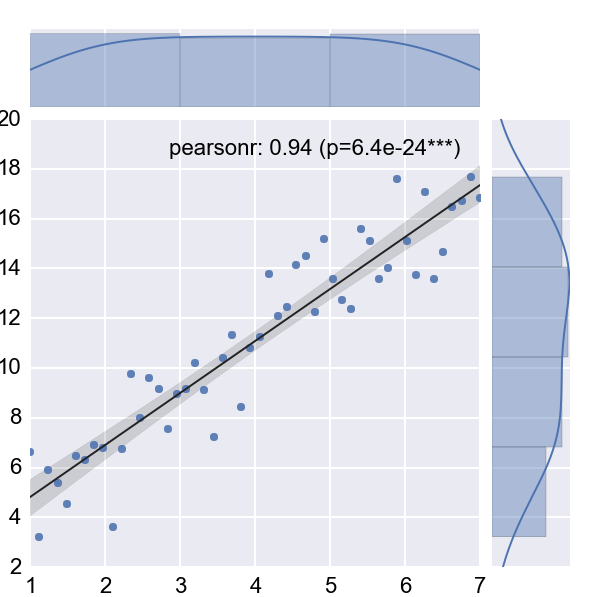
\includegraphics[width=0.5\textwidth]{../Images/regplot.png}\\
  \caption{Regression plot, from \emph{seaborn}, with a substantial amount of added information.}
\end{figure}

\subsection{General Routines}
Here is also a good place to introduce the short function that we will use a number of times to simplify the reading in of data:

\PyImg "getData.py" (p \pageref{py:getData}) Gets the input data for the Python programs in this script.
\index{python}{getData}

\section{Exercises}

\begin{itemize}
  \item Read in data from different sources:
  \begin{itemize}
    \item A CVS-file with a header ('Data\textbackslash Swimming\textbackslash swimming\_100m.csv')
    \item An MS-Excel file ('Data\textbackslash data\_dobson\textbackslash GLM\_data\textbackslash Table 2.8 Waist loss.xls')
    \item Data from the WWW (see "readZip.py" \ref{py:readZip})
  \end{itemize}
  \item
  \begin{itemize}
      \item Generate a pandas dataframe, with the x-column time stamps from 0 to 10 sec, at a rate of 10 Hz, the y-column data values with a sine with 1.5 Hz, and the z-column the corresponding cosine values. Label the x-column "Xvals", and the y-column "YVals", and the z-column "ZVals".
      \item Show the head of this dataframe
      \item Extract the data in lines 10-15 from "Yvals" and "ZVals", and write them to the file "out.txt".
  \end{itemize}
\end{itemize}
